The Alaskan rivers and streams are comprised of 5 species of salmon; sockeye \emph{O. nerka}, chinook \emph{O. tshawytscha}, coho \emph{O. kisutch}, chum \emph{O. keta}, and pink \emph{O. gorbuscha}.
Of the 5 species, sockeye salmon is the most common food source for Alaskan brown bears~\cite{ADFGsalmon}.
Sockeye salmon begin their journey hatching in streams and making their way down to the ocean.
At this point, they spend a year to 2 years out at sea before migrating back to the streams where they originated.
According to the National Park Service (NPS), only $25-40\%$ of returning salmon in Bristol Bay, Alaska, escape harvesting from commercial fisheries~\cite{NPS}.
They will then travel several miles upstream, where they lay and fertilize their eggs, called spawning.
Salmon will then lay between 1,500 to 10,000 eggs when spawning, but only 0 to 10 of these eggs will reach adulthood~\cite{WFRC}.
A significant proportion of energy for spawning salmon is spent reaching an optimal place to lay and fertilize their eggs, so much so that once they finish this process, they usually die shortly after~\cite{ADFGsalmon}. 

Based on the information above, the rate at which the salmon population grows appears to be exponential.
On average, for every salmon that lays eggs, 5 of their offspring will survive long enough to be adults ready to migrate back to their birthplace. Then, according to the NPS, approximately 32\% of those 5 offspring will make it past escapement to reproduce. These conditions allow us to model the salmon population, shown below,
\begin{equation}\label{eq:fishexpbase5}
    x(t) = x_0(0.32*5)^t,
\end{equation}
where $x_0$ is the initial number of salmon that laid eggs and $t$ represents time in years. We can then rewrite this exponential function with base $e$, as shown below,
\begin{equation}\label{eq:fishexp}
    x(t) = x_0e^{r_xt},
\end{equation}
where $r_x=\ln{(0.32*5)}$ represents the growth rate. Taking the derivative of $x(t)$ give us the salmon population's instantaneous rate of change,
\begin{equation}\label{eq:fishexpdif}
    \frac{dx}{dt} = r_xx_0e^{r_xt} = r_xx.
\end{equation}
% The above first order ordinary differential equation is now represented as the exponential growth model discussed in chapter 2. 
To examine the solution of the above model, we plot the function with an initial starting point of $20$.
% \begin{figure}[H]
%     \centering
%     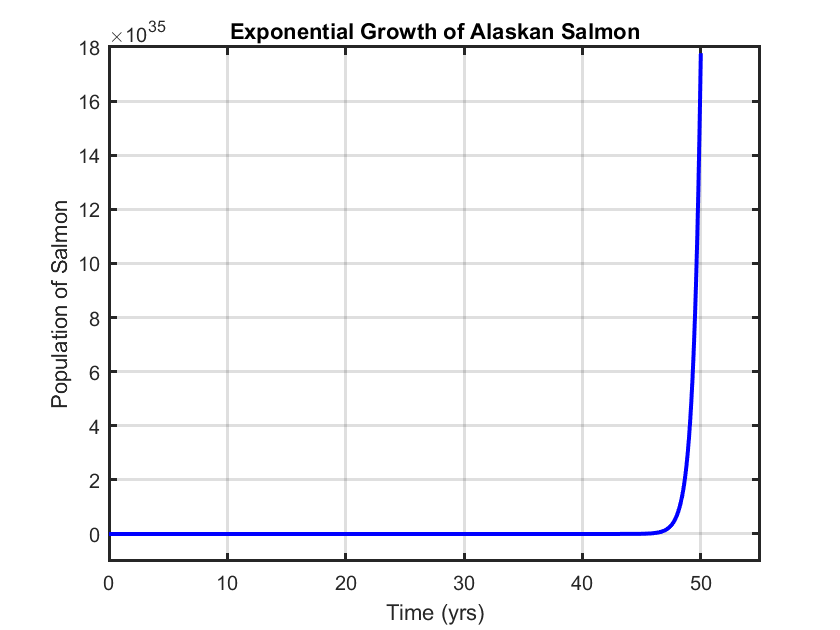
\includegraphics[width=14cm]{Pictures/Salmon Pop/Fish Exponential.png}
%     \caption{The plot above illustrates the population of salmon increasing exponentially resulting in a total of approximately \num{1.8e36} salmon after 50 years.}
%     \label{fig:salmonexp}
% \end{figure}
% Judging from the figure above the population appears quite small until around year 47.
% The population at the 47 year mark is approximately \num{5.7e32} salmon which is not small at all.
% To see this trend a little bit better the graph below is the same plot but for 2 years instead of 50.
\begin{figure}[H]
    \centering
    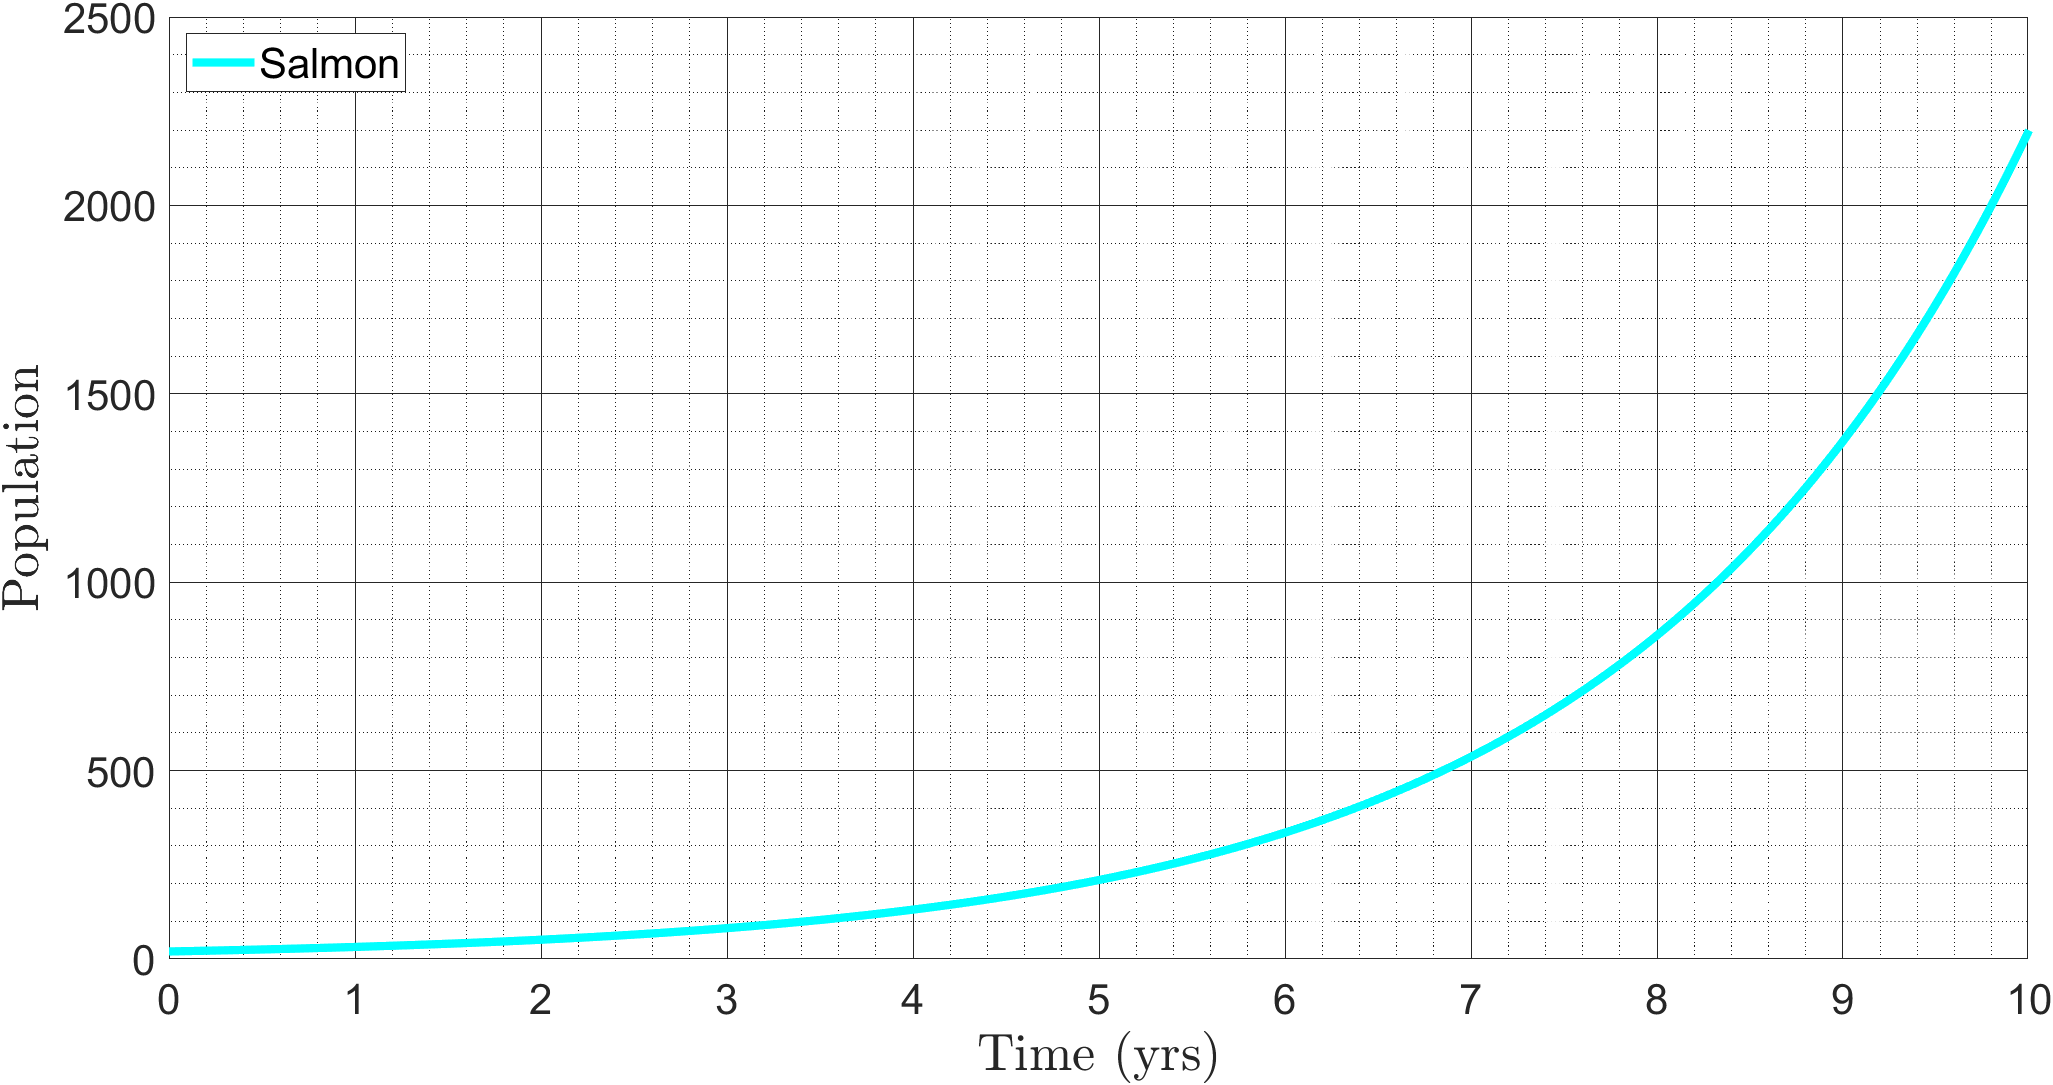
\includegraphics[width=14cm]{Pictures/Salmon Pop/SalmonExpo.png}
    \caption{\singlespacing
    Plot of the exponential growth model for the salmon population with respect to time.}
    \label{fig:salmonexpzoom}
\end{figure}
This figure illustrates that the population of salmon increases quickly in a short period.
In just 9 years, the population of salmon increases from 20 to approximately 1,400, and 1 year later, the population grows to about 2,200. 
The issue with this model is that the population gets extremely large in a short period of time, eventually reaching values that would fall well outside physical possibility.
Now that we have established a growth rate, a carrying capacity can be estimated using data from the ADFG in Bristol Bay, Alaska.

Bristol Bay is located on the easternmost side of the Bering Sea and is where many salmon migrate when returning home to reproduce.
There was a dramatic increase in sockeye salmon returning to Bristol Bay in 2021 compared to previous years. However the average weight of sockeye salmon this year decreased by a pound compared to the average for the past 20 years~\cite{bristol}.
% In Bristol Bay, there are 5 different species of salmon: sockeye \emph{O. nerka}, chinook \emph{O. tshawytscha}, coho \emph{O. kisutch}, chum \emph{O. keta}, pink \emph{O. gorbuscha} \cite{bristol}.
The sockeye species make up a large majority of the inshore runs, harvests\footnote{Harvests is defined as the number of fish gathered by commercial fisheries.}, and escapements\footnote{Escapements are salmon that escape the fisheries and continue upstream to spawn.} in Bristol Bay each year, which explains why the brown bear population mainly feeds on sockeye salmon~\cite{bristol}.
\begin{table}[H]
\rowcolors{2}{white!40}{lightgray!40}
    \centering
    \caption{Sockeye Comparison Between Weight and Run Size in Bristol Bay}\label{tab:weightvsrunshort}
    \vspace{.25cm}
    \begin{tabular}{|c|c|c|}
    \hline
         \textbf{Year} & \textbf{Weight (lbs)} & \textbf{Run (mil)} \\
    \hline
         2001 & 6.7 & 22.3\\
         2002 & 6.1 & 16.9\\
         2003 & 6.3 & 24.9\\
         2004 & 5.8 & 41.9\\
         \vdots & \vdots & \vdots\\
         2017 & 5.5 & 57.6\\
         2018 & 5.1 & 63.0\\
         2019 & 5.1 & 56.4\\
         2020 & 5.1 & 58.3\\
         2021 & 4.7 & 67.7\\
         \hline
    \end{tabular}
    \vspace{1ex}
    
    {\singlespacing
    % \raggedright 
    *This table gives a brief look at the relationship between run size and the average annual weight of sockeye salmon in Bristol Bay. 
    See \tablename~\ref{tab:runvsweight} in \appendixname~\ref{appendix:salmon} for the complete data.\par}
\end{table}
In the first 3 years of this table, the weight seems to be dramatically higher than in the last 3 years, but the opposite effect appears in run size.
This proposes the question that there might be a correlation between the run size and the average weight of salmon each year.
When taking a closer look at \tablename~\ref{tab:runvsweight} in \appendixname~\ref{appendix:salmon}, the trend becomes more apparent when comparing the sockeye's run size and the average annual weight.
Before calculating the correlation between these two events, we must create a plot to see if the trend is linear.
\begin{figure}[H]
    \centering
    \includegraphics[width=14cm]{Pictures/runVSweight/runVSweightNoTitle.png}
    \caption{\singlespacing
    Scatter plot of the variables; inshore run size and the average weight of salmon during that year's run, with the line of best fit.}
    \label{fig:runvsweight}
\end{figure}
Based on the figure above, there is a linear correlation between sockeye run size and their average weight.
The run size of the sockeye salmon decreases as their average weight increases. 
Since multiple variables make up the size of a salmon run each year, this helps explain the variance seen in the plot.
So, calculating the correlation of these two events gives a value of $-0.88$.
Since the correlation of these events is strong, an environmental limit of salmon can be estimated based on the maximum annual volume of sockeye salmon for the past 21 years.
When looking at \tablename~\ref{tab:volume} in \appendixname~\ref{appendix:salmon}, the maximum volume for any given run in the last 21 years was $7.34$ million cubic feet (MMCF) in $2018$. 
The average weight of sockeye salmon during this year was $5.1$ lbs, which is $0.4$ lbs more than the lowest average weight of $4.7$ lbs in 2021.
Now, the carrying capacity for sockeye salmon can be estimated using the maximum volume and the lowest average weight, producing a value of $68.4$ million sockeye salmon.
Sockeye are not the only salmon in the river streams, but according to 
\tablename~\ref{tab:harvestBristol} in \appendixname~\ref{appendix:salmon}, they make up approximately $94\%$ of the average annual commercial harvest in Bristol Bay.
Assuming that the run proportions are the same as the average annual commercial harvest, $72.8$ million becomes the carrying capacity for inshore salmon runs in Bristol Bay.
As stated earlier, approximately 32\% of adult salmon will escape commercial harvesting, which changes the carrying capacity to $29.1$ million salmon each year~\cite{NPS}.


Now that we have the carrying capacity of the salmon population, we can construct their logistic growth model to be
\begin{equation}\label{eq:fishlogistic}
    \frac{dx}{dt} = r_xx\left(1-\frac{x}{K_x}\right),
\end{equation}
where $K_x=29,100,000$ is the carrying capacity, and $r_x=\ln{(0.32*5)}$ is the growth rate.
If we start with an initial population of $20$ million, the population should have the below trend.
\begin{figure}[H]
    \centering
    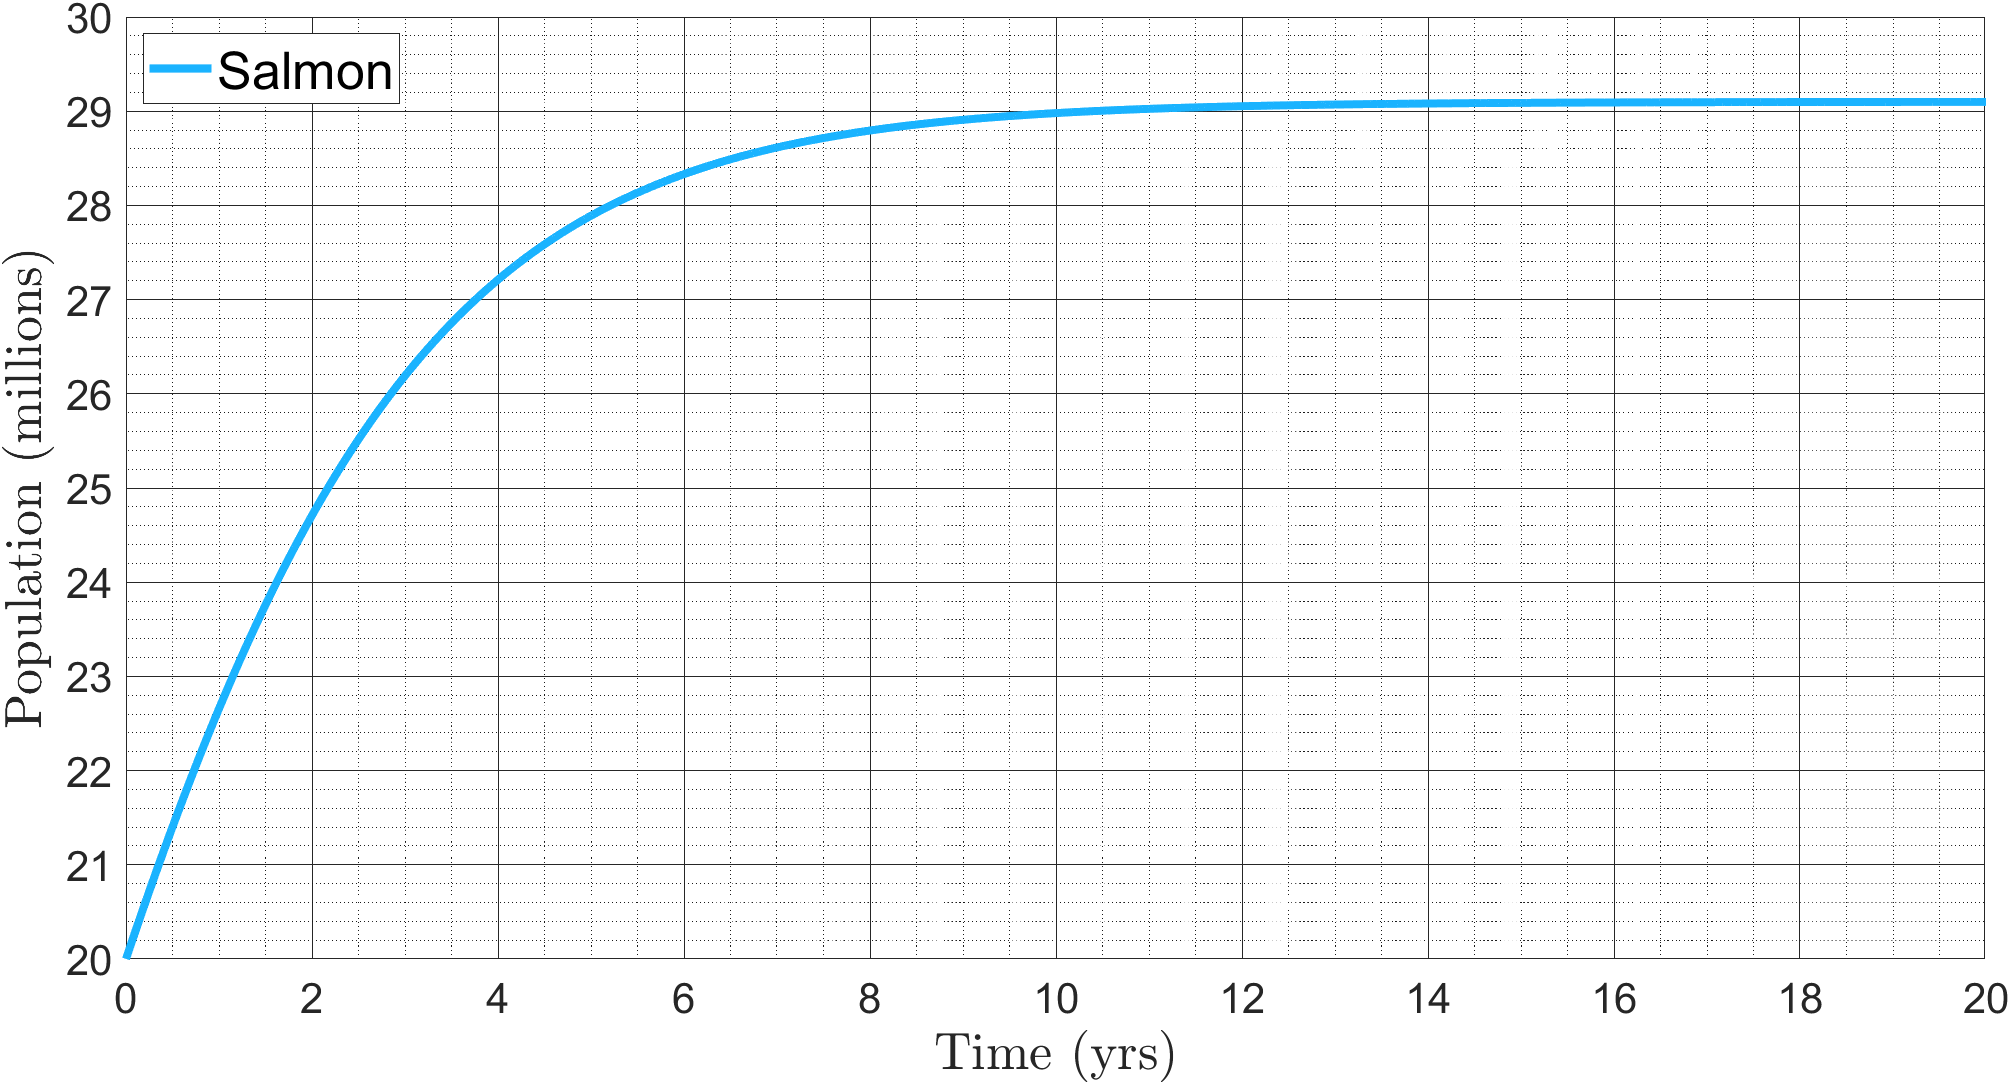
\includegraphics[width=14cm]{Pictures/Salmon Pop/SalmonLogistic.png}
    \caption{\singlespacing
    Plot of the logistic growth model for the salmon population with an initial population of $20$ million.}
    \label{fig:salmnologistic}
\end{figure}
From the graph above, the population of salmon grows rapidly for about 14 years before approximately reaching the carrying capacity.
In the next chapter, we will examine if the changes in temperature affect the growth rate of salmon, and if so, incorporate climate change into the model and evaluate the results.



% Cooper Creek, Kenai River, Russell Creek, Terror River, and Staney Creek





% \begin{itemize}
%     \item Pacific coast salmon lay between 1500 to 10000 eggs.
%     \item 0 to 10 survive to adult hood
%     \item According to the Alaskan government the population of sockeye Salmon follow a logistic curve for each year.
%     \item They grow exponentially but there is a carrying capacity.
% \end{itemize}